% ProLiVis 2.0 — supplementary material
%
% Build:  tectonic -X compile supplement.tex
% Figures and tables are generated: cd ../web && npm run supplement
%
% Single column, unlike the manuscript: this document is mostly screenshots of a
% wide interface, and a two-column measure would print them at postage-stamp size.
\documentclass[11pt,a4paper]{article}

\usepackage[T1]{fontenc}
\usepackage[margin=2.3cm]{geometry}
\usepackage{graphicx}
\usepackage{booktabs}
\usepackage{microtype}
\usepackage{url}
\usepackage[hidelinks]{hyperref}
\usepackage{caption}
\captionsetup{font=small}

% Generated by tests/figures/supplement.spec.ts. Do not edit.
\newcommand{\SuppUpset}{%
  Proximity Label-MS & 15{,}456 \\
  Affinity Capture-MS & 8{,}124 \\
  Affinity Capture-MS + Proximity Label-MS & 3{,}779 \\
  Co-fractionation & 1{,}684 \\
  Protein-RNA & 1{,}013 \\
  Affinity Capture-RNA & 512 \\
  Protein-peptide & 480 \\
  PCA & 378 \\
}
\newcommand{\SuppTimeline}{%
  Proximity Label-MS & 26{,}776 & 2020 \\
  Affinity Capture-MS & 16{,}970 & 2021 \\
  Co-fractionation & 2{,}027 & 2025 \\
  Protein-RNA & 1{,}650 & 2023 \\
  Affinity Capture-RNA & 1{,}614 & 2023 \\
  Reconstituted Complex & 1{,}361 & 2021 \\
}
\newcommand{\SuppChord}{%
  Affinity Capture-MS & Proximity Label-MS & 4{,}243 \\
  Affinity Capture-MS & Protein-RNA & 365 \\
  Affinity Capture-MS & Co-fractionation & 263 \\
  Affinity Capture-MS & Affinity Capture-Western & 243 \\
  Protein-RNA & Proximity Label-MS & 222 \\
  Affinity Capture-MS & Affinity Capture-RNA & 221 \\
  Affinity Capture-MS & Two-hybrid & 192 \\
  Co-fractionation & Proximity Label-MS & 174 \\
}
\newcommand{\SuppInteractions}{34{,}540}
\newcommand{\SuppProteins}{8{,}510}
\newcommand{\SuppYearFirst}{2004}
\newcommand{\SuppYearLast}{2025}
\newcommand{\SuppBipartiteNodes}{212}
\newcommand{\SuppBipartiteLinks}{1{,}511}
\newcommand{\SuppBipartiteLanes}{3}
\newcommand{\SuppRelease}{5.0.260}
\newcommand{\SuppRecords}{76{,}632}


\title{ProLiVis 2.0 --- Supplementary Material\\[2pt]
\large A walkthrough of every capability}
\author{Melih Sozdinler}
\date{}

\begin{document}
\maketitle

\section{What this document is}

The manuscript argues one thing: that a protein interaction database records evidence
without weighing it, and that a literature-centric view with a trust model on every
edge makes the difference visible. This supplement is the other half --- what the tool
actually does, capability by capability, with a figure for each.

Everything shown here comes from BioGRID release \SuppRelease{}, the coronavirus file
(\SuppRecords{} records, 4.5\,MB), restricted to SARS-CoV-2 unless stated: a reader can
download it and reproduce every figure. Where a capability only means something at
scale, the manuscript reports the full release instead.

Figures and tables are generated rather than assembled by hand:

\begin{verbatim}
  cd web
  PROLIVIS_FIGURE_SOURCE=~/Downloads/BIOGRID-CORONAVIRUS-5.0.260.tab3.zip \
    npm run supplement
\end{verbatim}

\paragraph{Interface or API.} ProLiVis has two surfaces, and this document is explicit
about which one each capability lives on. The interface is what a browser tab shows.
The scripting API is \texttt{window.prolivis}, available in any browser console and in
headless automation; it is a supported interface, not a debugging hook --- the tool's
own tests and every figure in the manuscript are produced through it. Table~\ref{tab:surfaces}
is the map. Four view models are computed but not yet drawn (\S\ref{sec:undrawn}); we
would rather say so than imply otherwise.

\begin{table}[h]
  \centering
  \small
  \caption{Where each capability lives.}
  \label{tab:surfaces}
  \begin{tabular}{lll}
    \toprule
    Capability & Interface & Scripting API \\
    \midrule
    Ingest a BioGRID file            & yes & \texttt{load}, \texttt{inspect} \\
    Online mode (BioGRID REST)       & no  & \texttt{connect}, \texttt{fetchRemote} \\
    Literature (center) view         & yes & \texttt{centerLayout}, \texttt{centerScene} \\
    Filter the literature            & yes & arguments to \texttt{centerLayout} \\
    Protein network, five layouts    & yes & \texttt{graph}, \texttt{networkLayout} \\
    Modules view and drill-down      & yes & \texttt{autoContract}, \texttt{highLevelLayout} \\
    Adjacency matrix                 & yes & \texttt{matrix} \\
    Trust threshold                  & yes & \texttt{score} \\
    Trust weights and presets        & no  & \texttt{trustPresets}, \texttt{gather}, \texttt{rescore} \\
    Calibration and ablation         & no  & \texttt{calibrate}, \texttt{ablate} \\
    Graph algorithms                 & no  & \texttt{cliques}, \texttt{modules}, \texttt{cores}, \dots \\
    Literature search and collection & yes & \texttt{findPublications}, \texttt{derive} \\
    Compare and merge                & yes & \texttt{compare}, \texttt{merge} \\
    Export a figure as SVG           & yes & \texttt{toSvg} \\
    Export data (CSV, GraphML, SIF)  & no  & \texttt{exportTable}, \texttt{exportGraphml}, \dots \\
    Session manifest                 & no  & \texttt{manifest}, \texttt{parseManifest} \\
    UpSet, timeline, chord, bipartite & no & \texttt{upset}, \texttt{timeline}, \dots \\
    \bottomrule
  \end{tabular}
\end{table}

\clearpage
\section{Getting data in}

\begin{figure}[h]
  \centering
  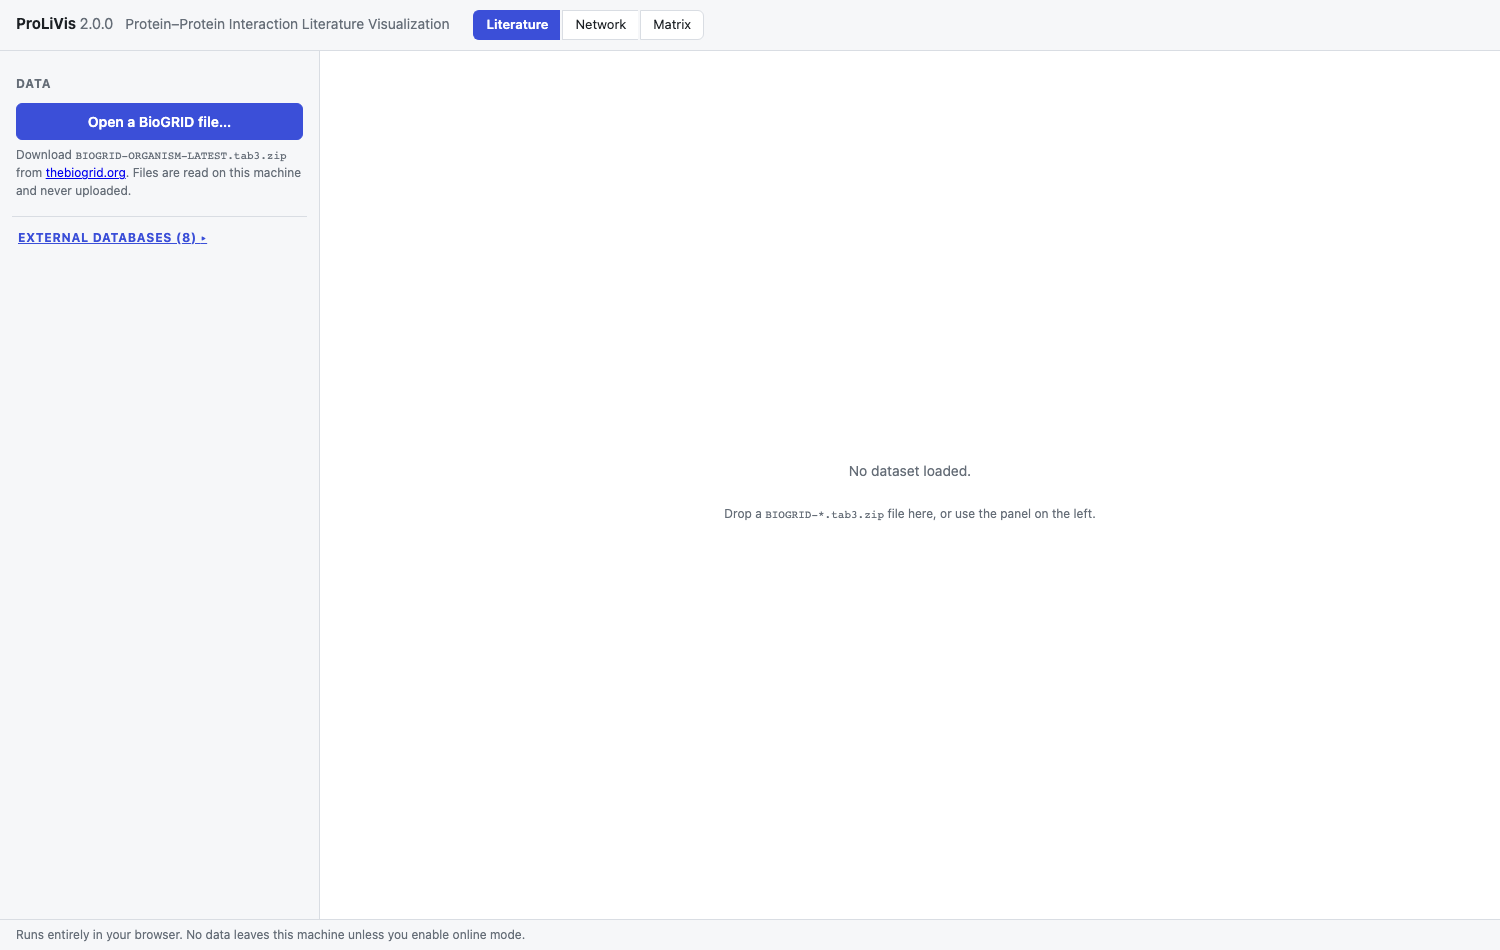
\includegraphics[width=0.86\textwidth]{supplement/empty.png}
  \caption{The application before any data. There is no account, no server and no
  upload: a BioGRID archive is opened from disk and parsed in the browser. The panel
  says where to get one.}
\end{figure}

A dropped \texttt{.tab3.zip} is inflated in line-aligned chunks with the reader
throttled, so peak memory is bounded by one chunk rather than by the archive; members
are listed first, and an archive holding one file per organism asks which. Columns are
resolved by alias onto a canonical set, because the bulk \texttt{tab3} files and the
\texttt{tab2} output of the REST service name six columns differently. The result is
stored in DuckDB compiled to WebAssembly and persisted in the browser's Origin Private
File System, so a second visit opens immediately; if the browser refuses persistent
storage --- a private window, or a second tab already holding the database --- the
application says so and continues in memory rather than failing.

\clearpage
\section{The literature view}

\begin{figure}[h]
  \centering
  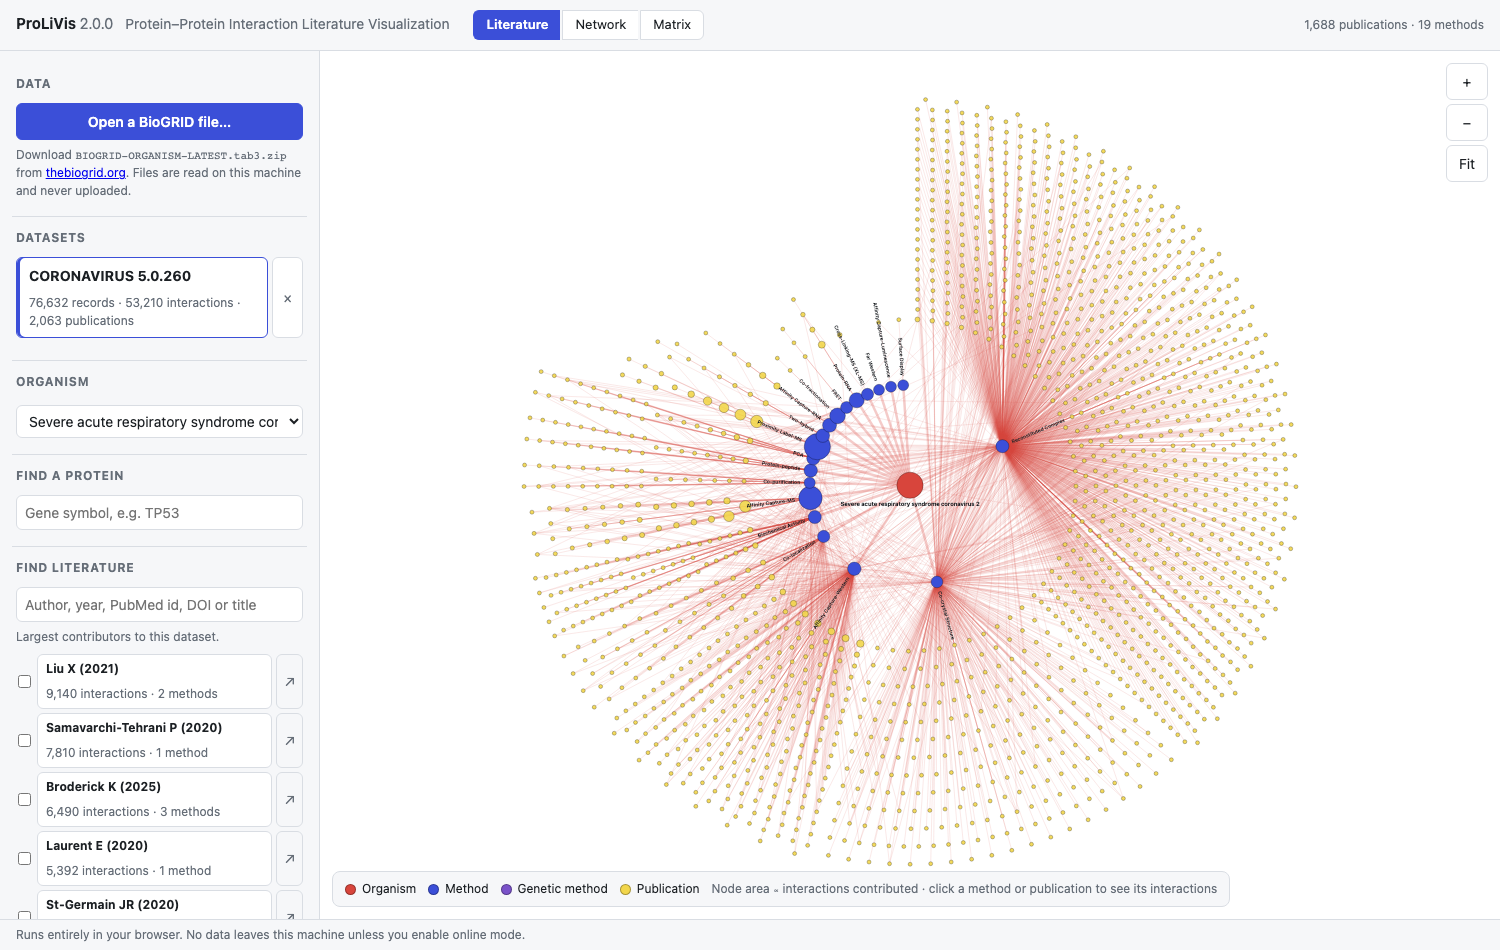
\includegraphics[width=0.86\textwidth]{supplement/literature.png}
  \caption{Center Layout 2.0 for SARS-CoV-2. The organism is at the centre,
  experimental methods form the inner ring, and publications fan outward within their
  method's sector. Sector width is share of the literature; node area is interactions
  contributed. Genetic methods are drawn in a different colour, because a genetic
  interaction is not a physical one.}
\end{figure}

\begin{figure}[h]
  \centering
  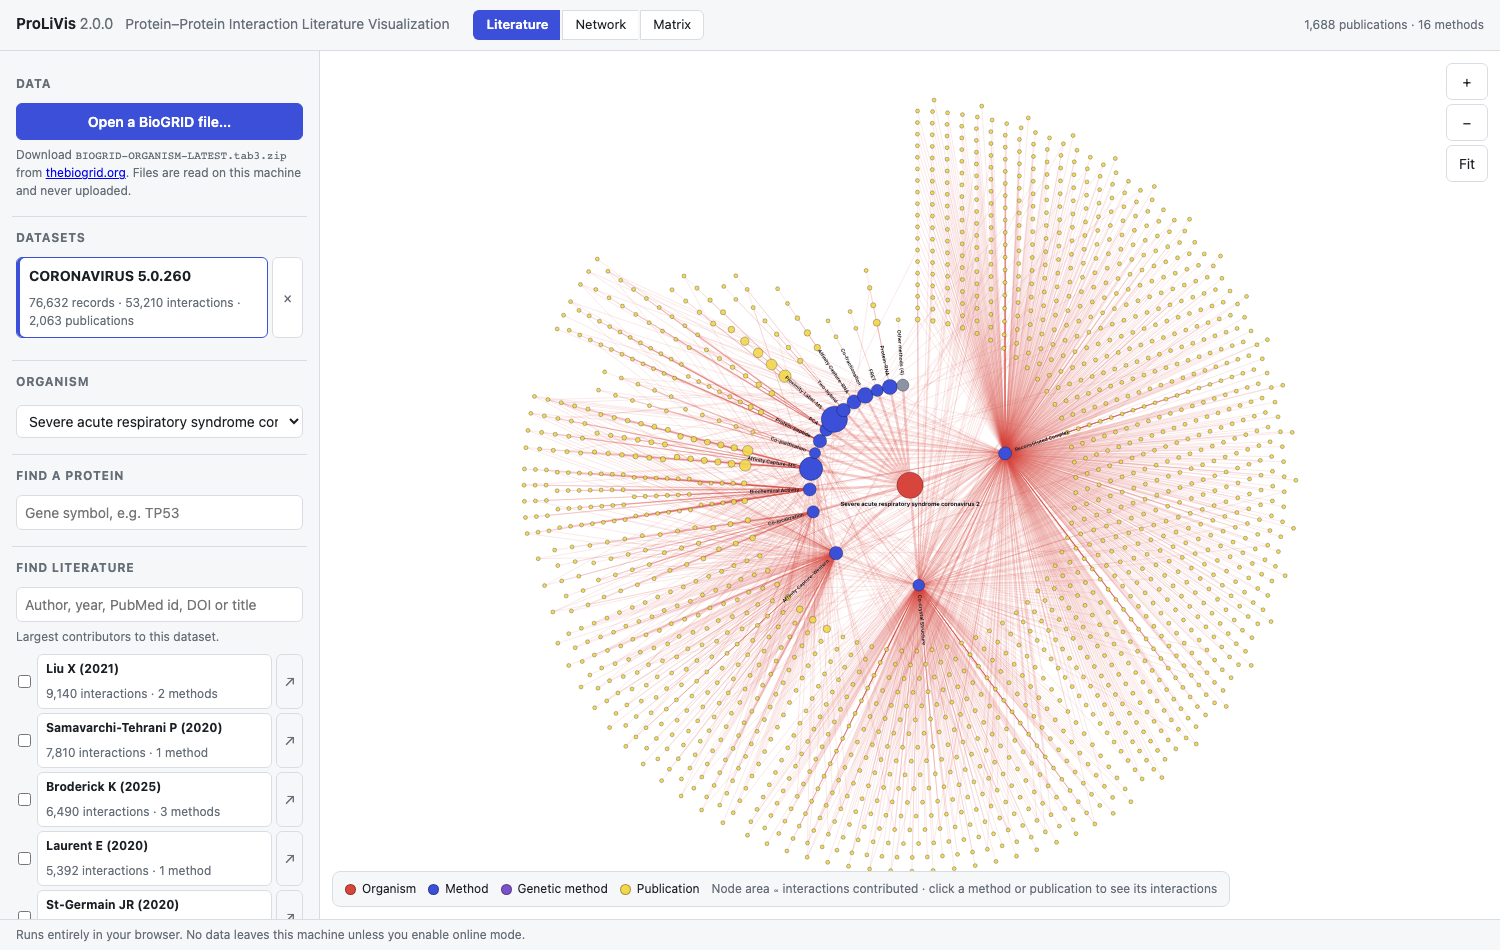
\includegraphics[width=0.86\textwidth]{supplement/literature-folded.png}
  \caption{The same literature with methods supported by fewer than five publications
  folded into a single node --- the paper's third level. The long tail otherwise
  consumes half the circle in slivers too thin to read or click.}
\end{figure}

\clearpage
\section{Filtering the literature}

Every publication is one node whatever it reported, so a screen contributing ten
thousand interactions and a structure paper contributing one look alike until you ask.
Three filters ask: contribution, proteins touched, and method.

\begin{figure}[h]
  \centering
  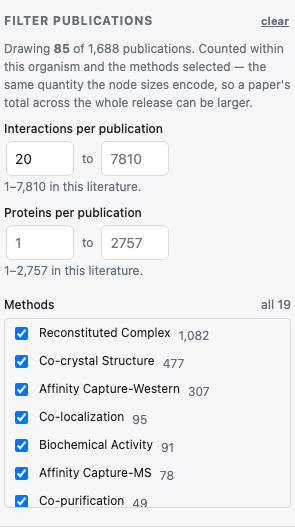
\includegraphics[width=0.46\textwidth]{supplement/filter-panel.png}
  \hfill
  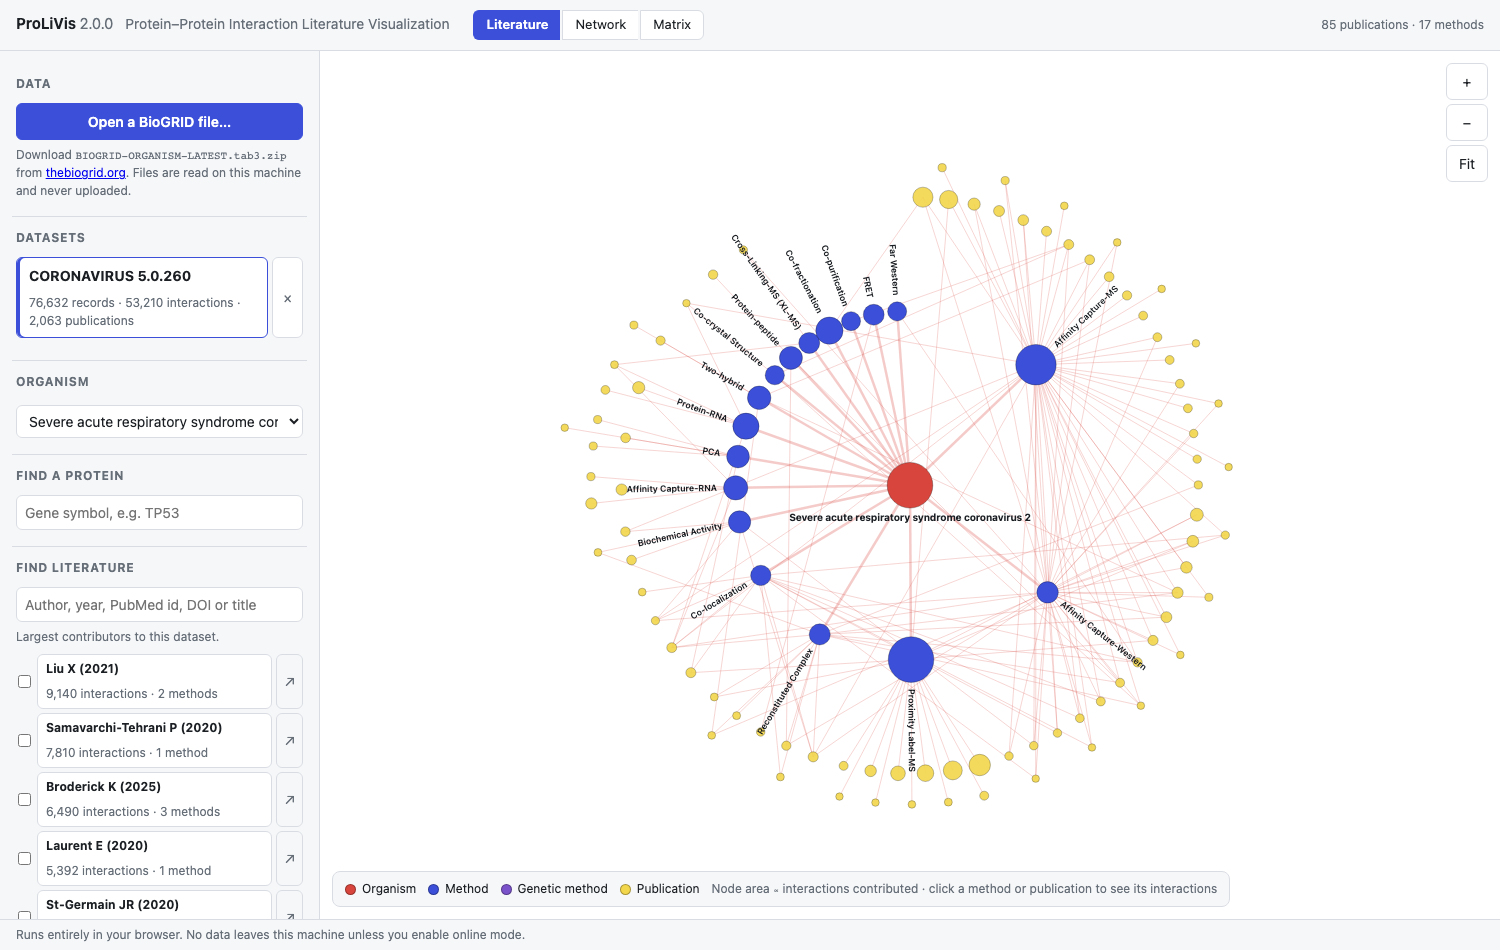
\includegraphics[width=0.5\textwidth]{supplement/literature-filtered.png}
  \caption{The filter, and its effect. Bounds beside each box are the range of the
  unfiltered literature, so they stay put as the view narrows. Counts are within the
  selected organism and methods --- the same quantity the node areas encode. Filtering
  recomputes the method ring from the publications that survive, since a sector's width
  is its share of the literature and a sector sized by papers that are no longer drawn
  would describe a different picture.}
\end{figure}

The publication band is bounded, so a literature larger than it holds is not drawn in
full; the panel reports what it drew against what exists, and what matched but did not
fit. This matters at scale rather than here: the human literature of this release is
41{,}218 publications, of which 16{,}148 fit.

\clearpage
\section{From a publication to what it reported}

\begin{figure}[h]
  \centering
  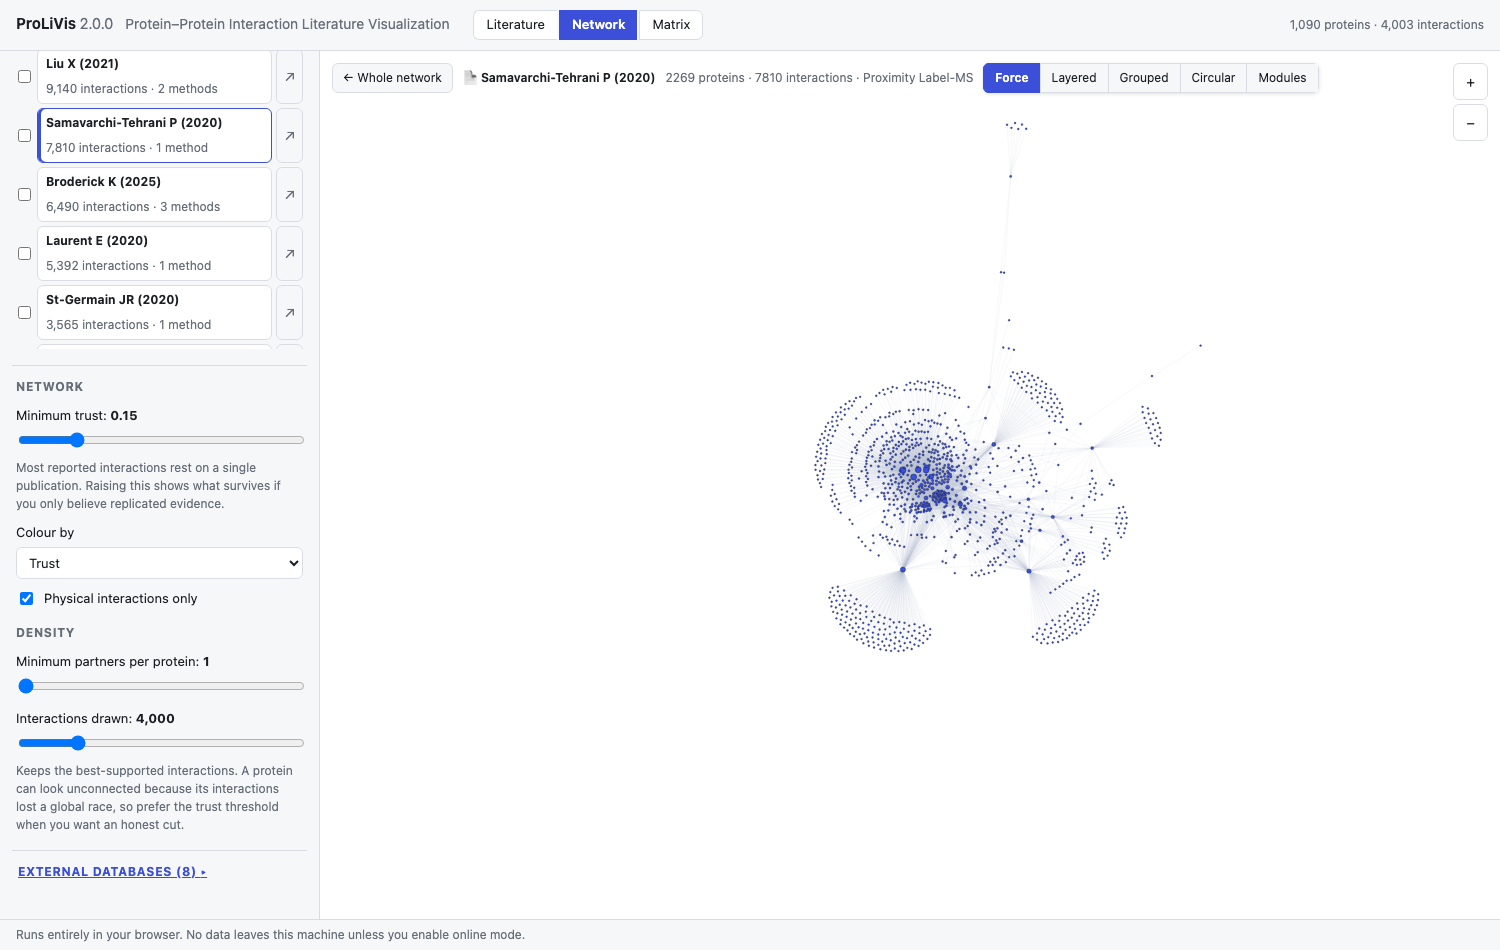
\includegraphics[width=0.86\textwidth]{supplement/publication-network.png}
  \caption{Clicking a publication node opens the interactions that paper reported. The
  breadcrumb above the canvas names the scope and returns to the whole network. A
  method node does the same one level up: every interaction that technique produced.
  Inside a scope the trust threshold does not apply --- you asked for a specific bounded
  set --- so trust shows as edge colour and weight instead of hiding anything.}
\end{figure}

\clearpage
\section{The protein network}

The figures below are the same network under each arrangement: SARS-CoV-2 at trust
$\geq 0.4$, keeping proteins with at least two partners and the 400 best-supported
interactions --- 48 proteins and 248 interactions. That is a deliberate choice for this
document. The whole organism is \SuppProteins{} proteins and \SuppInteractions{}
interactions, and a figure of that says only ``it is large''; what an arrangement
\emph{means} is legible at fifty nodes.

\begin{figure}[h]
  \centering
  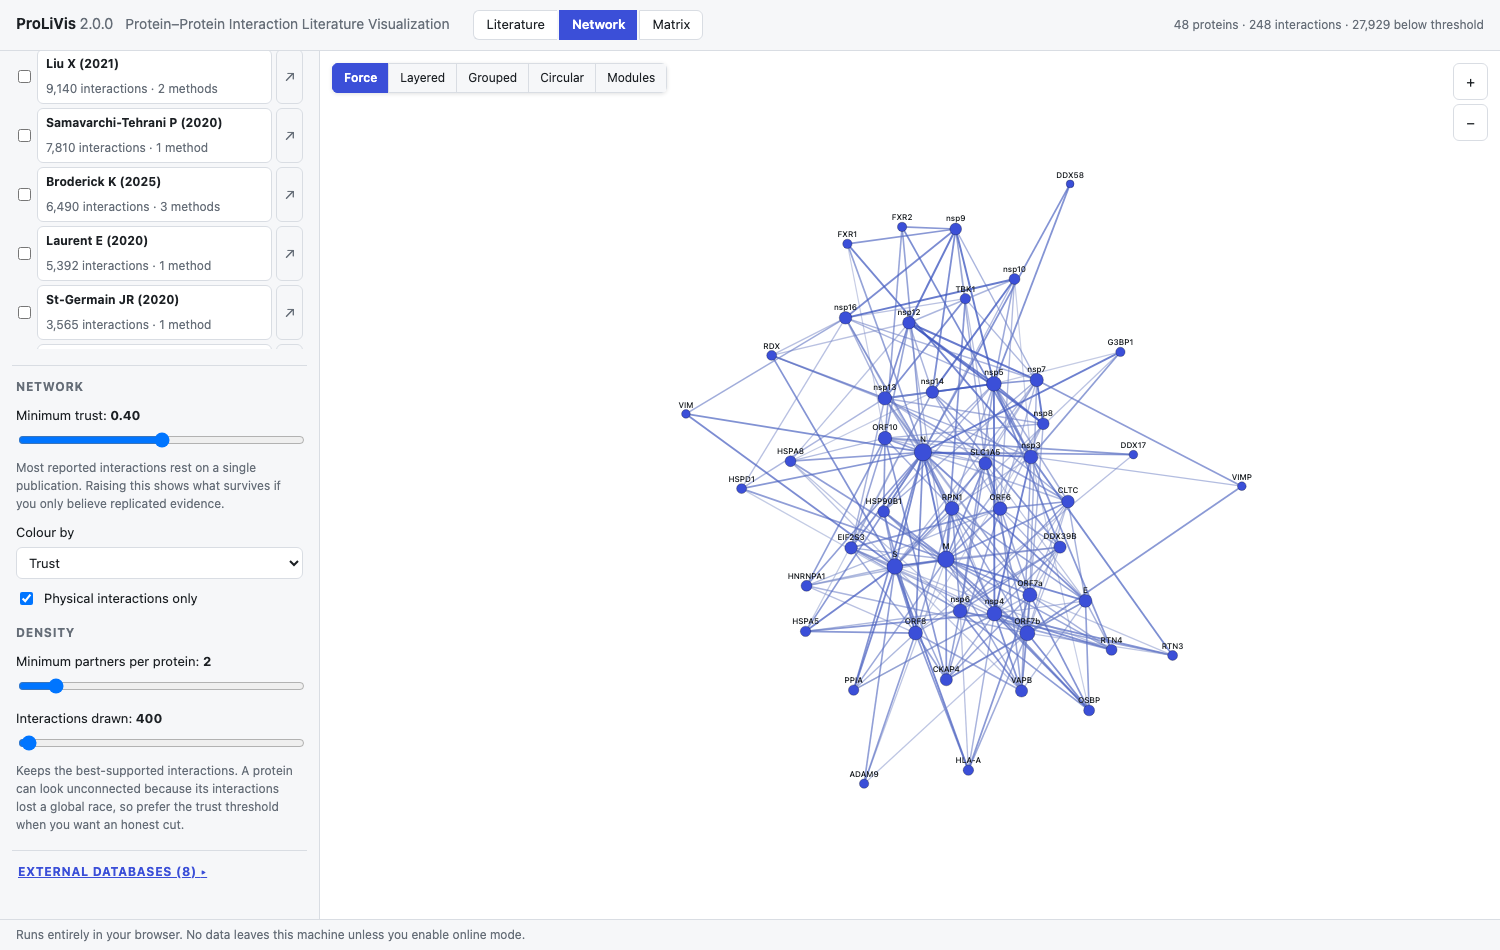
\includegraphics[width=0.86\textwidth]{supplement/network-force.png}
  \caption{Force. What clusters together. The replication machinery (nsp5, nsp9, nsp10,
  nsp12--nsp16) sits together, with host chaperones and stress-granule proteins
  (HSPA5, HSPA8, G3BP1, DDX58) around it. The density controls used are on the left;
  the header reports how many interactions the threshold hid.}
\end{figure}

\begin{figure}[h]
  \centering
  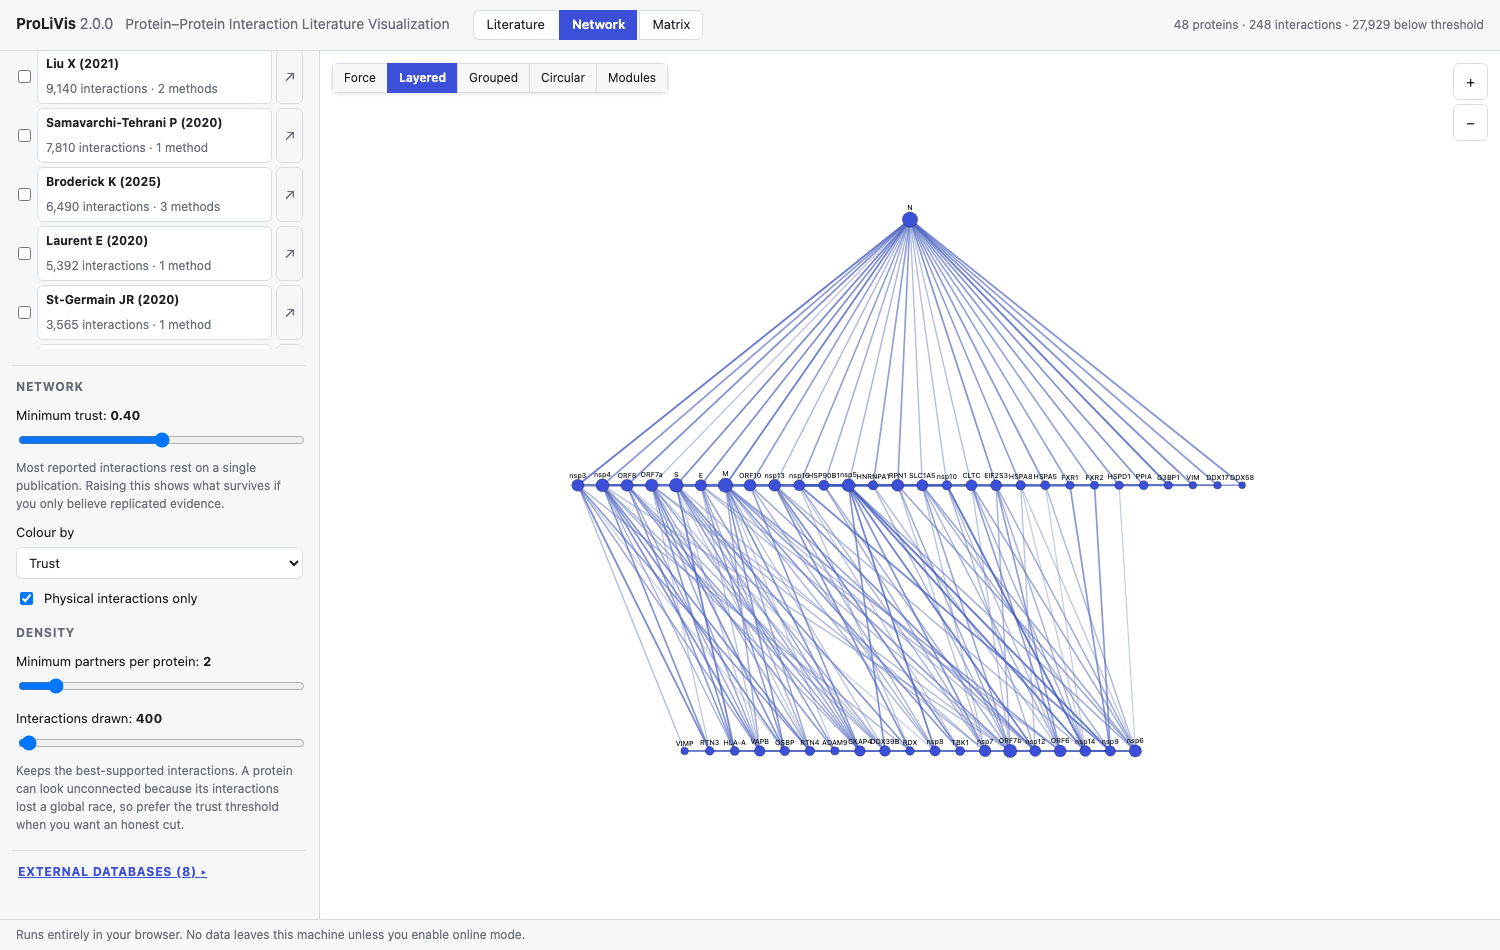
\includegraphics[width=0.86\textwidth]{supplement/network-layered.png}
  \caption{Layered. Vertical position is graph distance from the best-connected
  protein, so ``how many hops apart are these'' can be read off the picture. Layers
  wider than the canvas wrap into sub-rows rather than overflowing.}
\end{figure}

\begin{figure}[h]
  \centering
  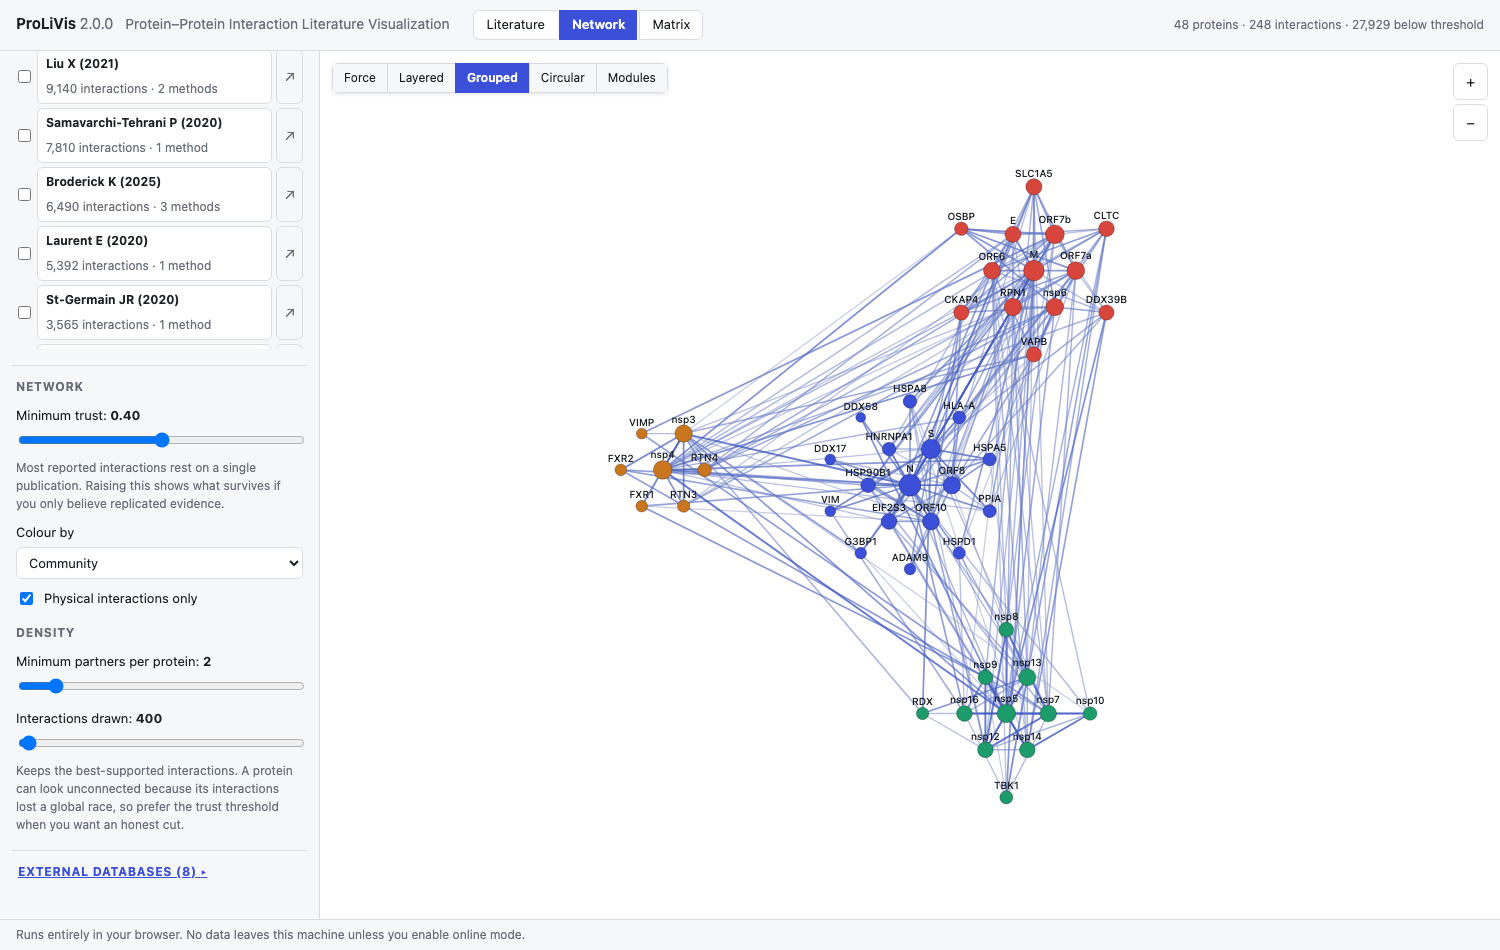
\includegraphics[width=0.86\textwidth]{supplement/network-grouped.png}
  \caption{Grouped, coloured by community. Trust-weighted communities as discs, packed
  around the largest, best-connected member at the centre of each. Grouping by
  connected component, the obvious choice, does not work here: a PPI network is one
  component, so every protein lands in one group and the arrangement draws a single
  disc.}
\end{figure}

\begin{figure}[h]
  \centering
  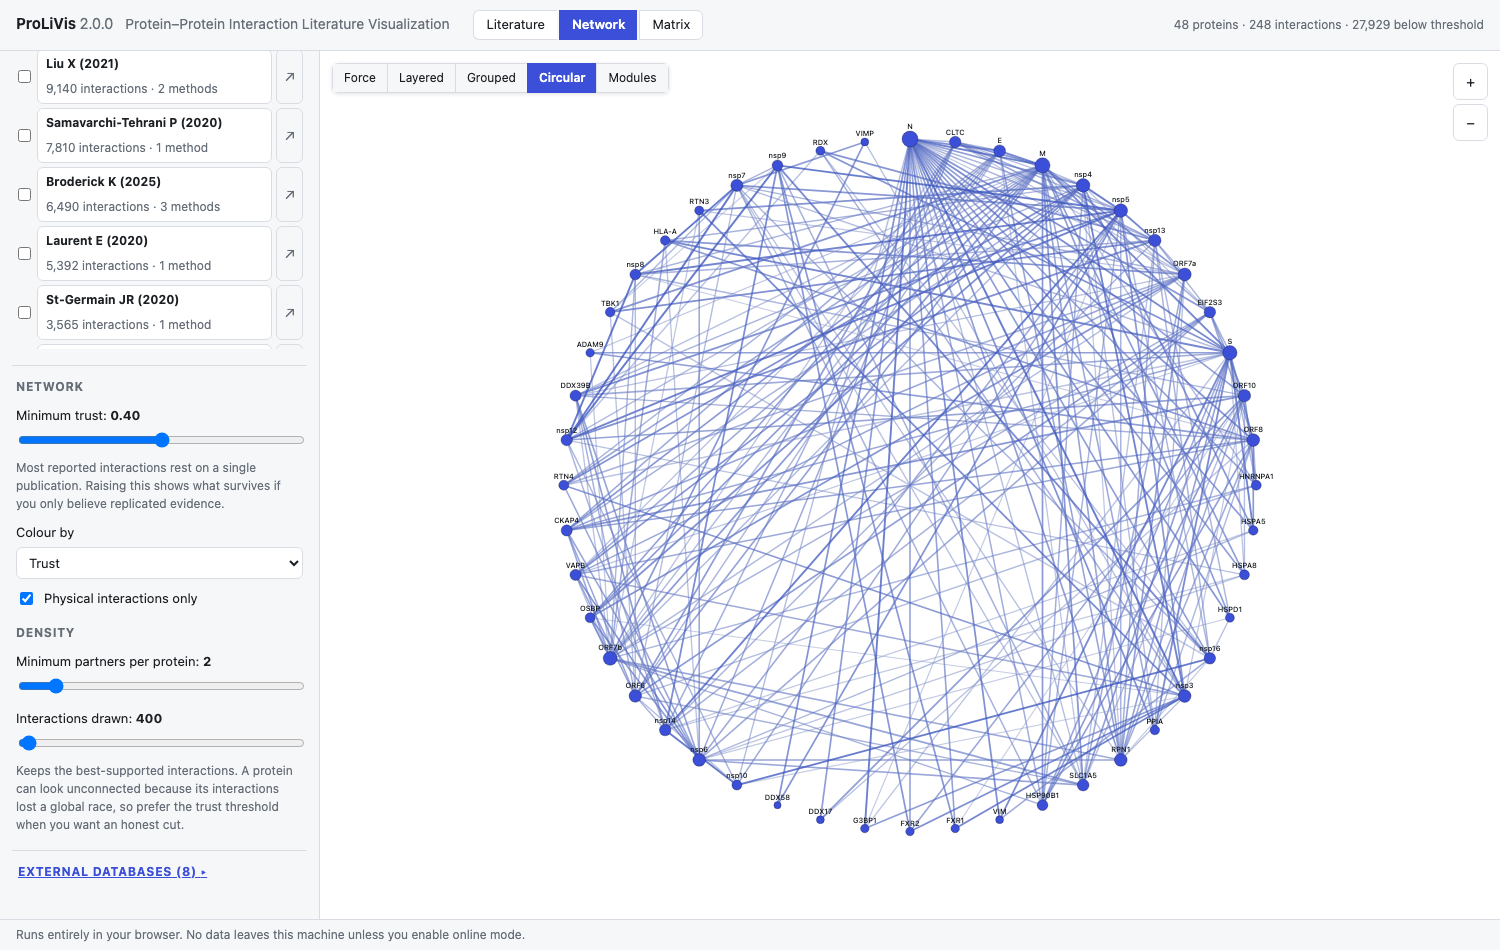
\includegraphics[width=0.86\textwidth]{supplement/network-circular.png}
  \caption{Circular. Everything on one ring, ordered by a traversal so neighbours sit
  together: a stable reference arrangement that makes no claim about structure.}
\end{figure}

The four arrangements are all deterministic: a seeded generator, a fixed iteration
count rather than a run to convergence, and locale-independent tie-breaking, so the
same network always draws the same picture and a figure can be regenerated from a
session manifest.

\begin{figure}[h]
  \centering
  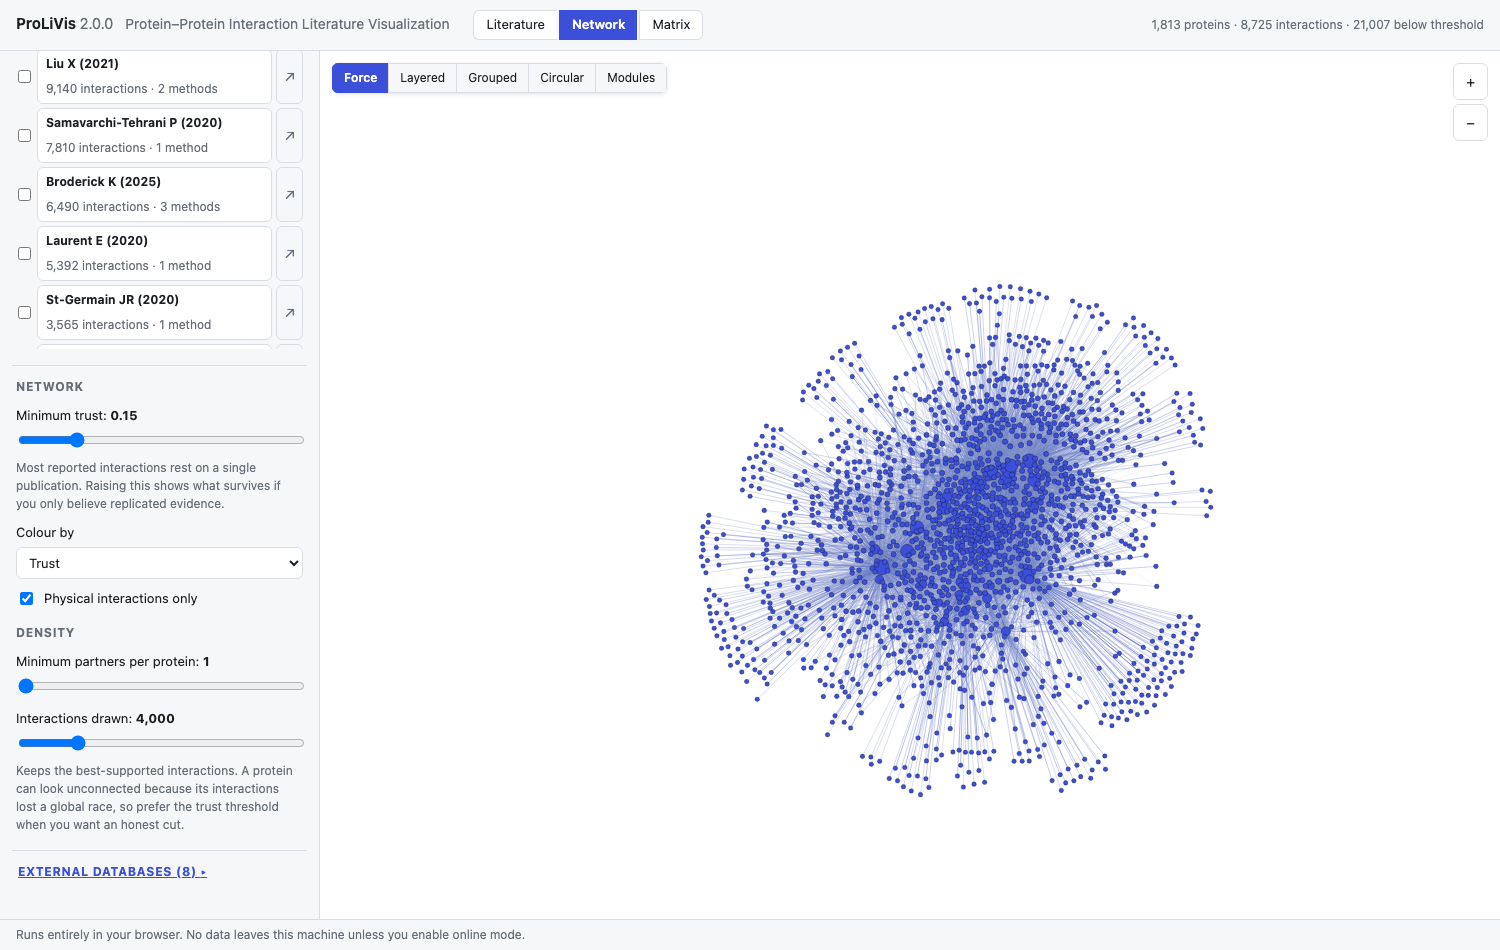
\includegraphics[width=0.49\textwidth]{supplement/network-force-large.png}
  \hfill
  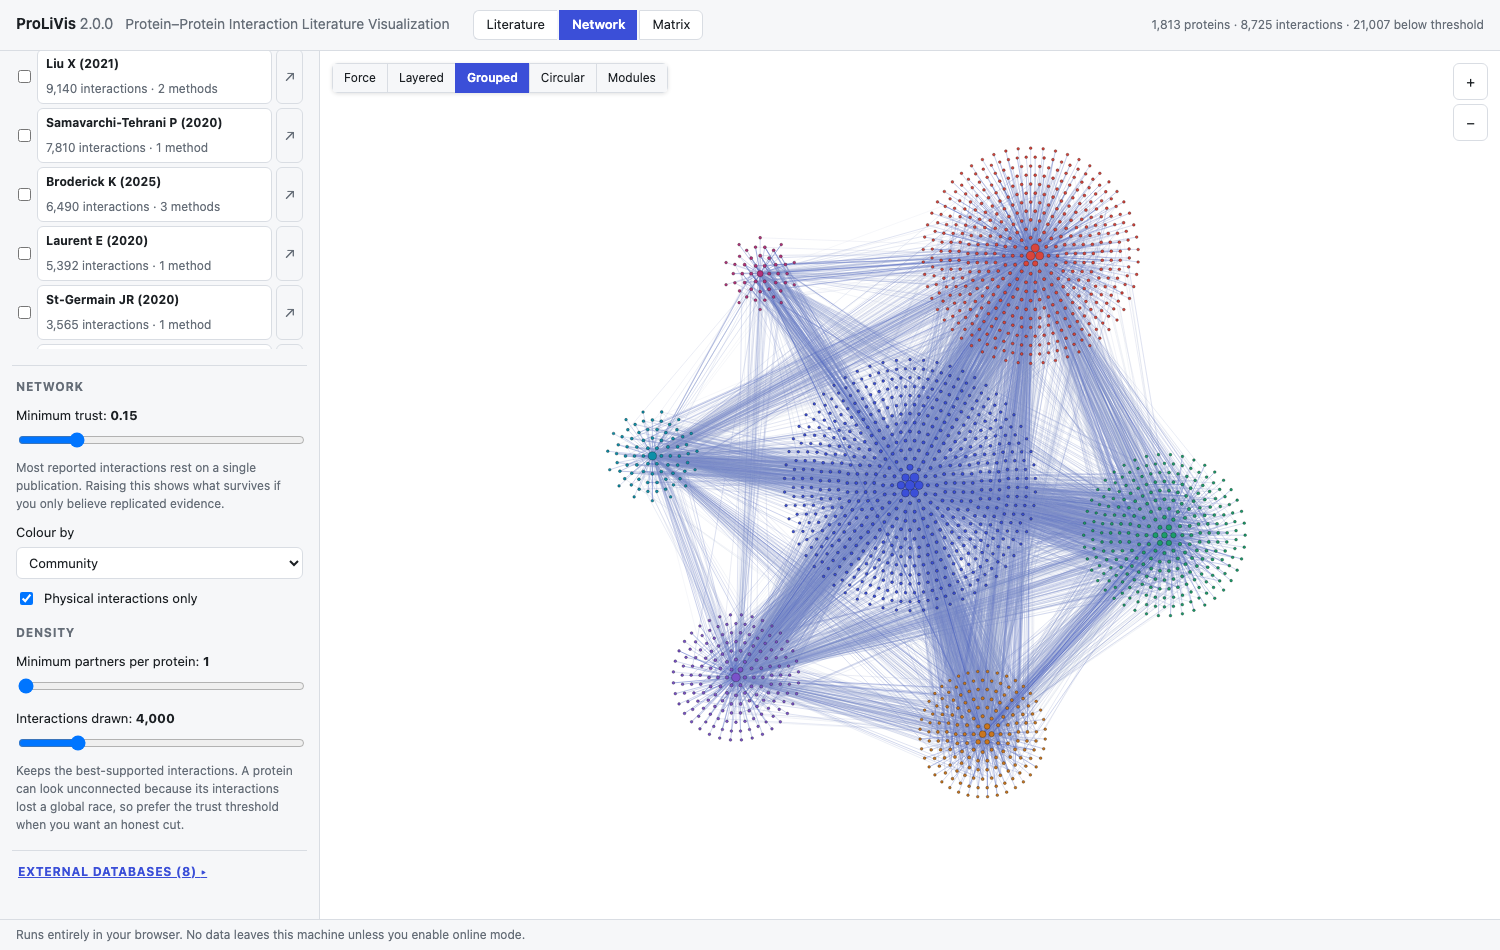
\includegraphics[width=0.49\textwidth]{supplement/network-grouped-large.png}
  \caption{The whole organism at the default threshold --- 1{,}813 proteins and 8{,}725
  interactions --- under Force (left) and Grouped (right). Force uses Barnes--Hut
  repulsion above three hundred proteins, which is what lets it draw a network this
  size at all; with exact repulsion it is a second's work only to about twelve
  hundred. At this size the force layout says how dense the network is and little
  else, which is what the modules view (\S\ref{sec:modules}) is for.}
\end{figure}

\begin{figure}[h]
  \centering
  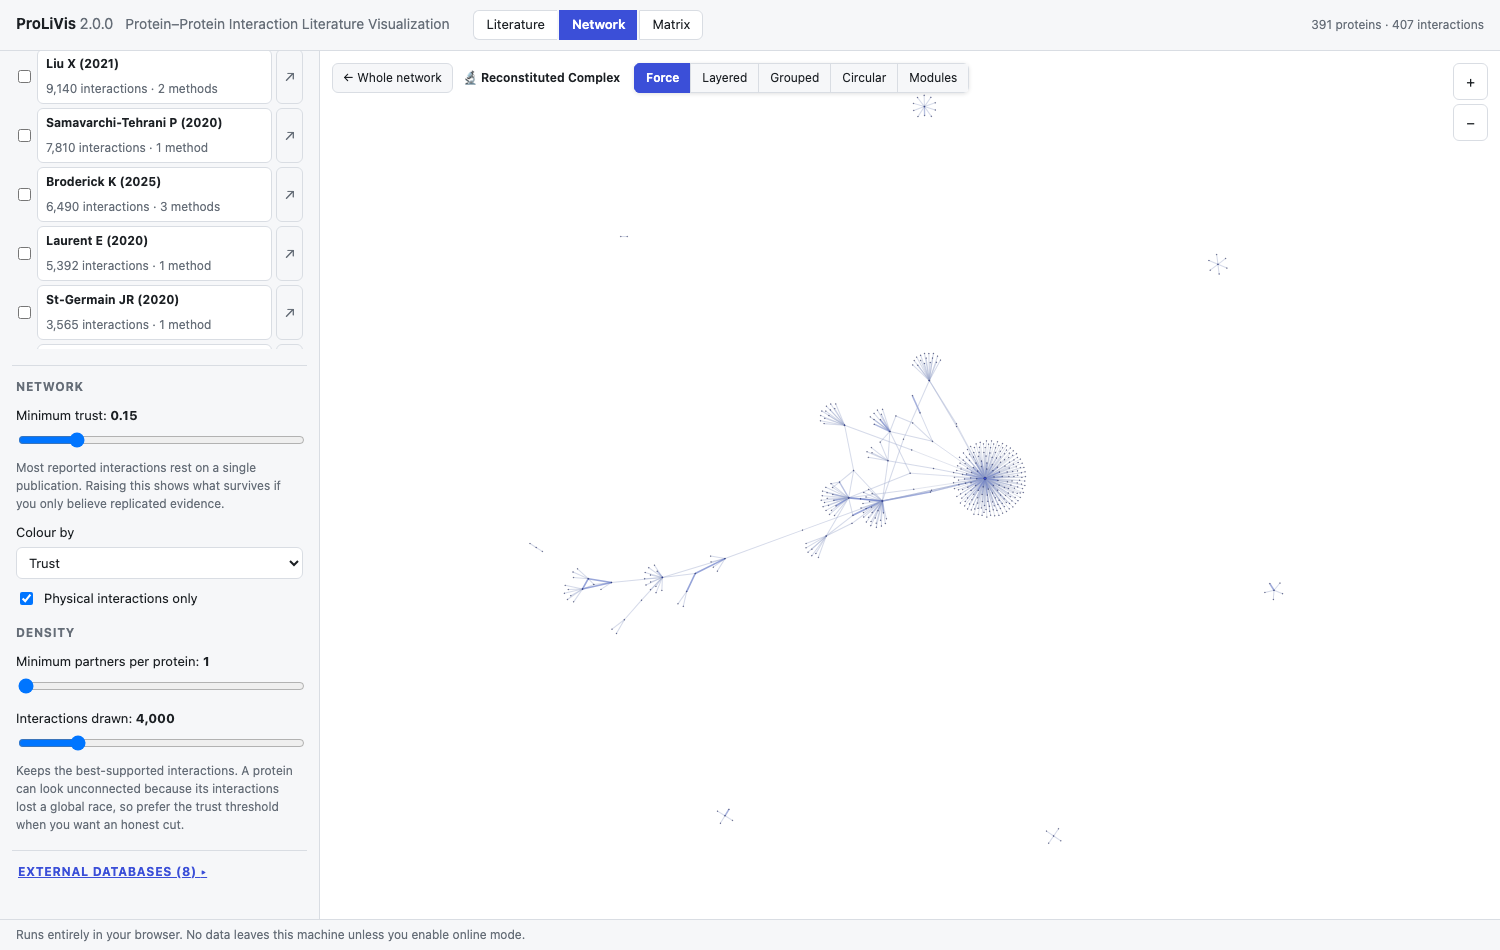
\includegraphics[width=0.86\textwidth]{supplement/network-sparse.png}
  \caption{A sparse network: everything reported by Reconstituted Complex, which falls
  into many components. Each is laid out on its own and they are packed around the
  largest, spread evenly. Left to one embedding, a component with no edge to the rest
  feels only repulsion and drifts far outside the others, so fitting the view to
  include it shrinks the part worth looking at.}
\end{figure}

\clearpage
\section{One protein, and the evidence behind it}

\begin{figure}[h]
  \centering
  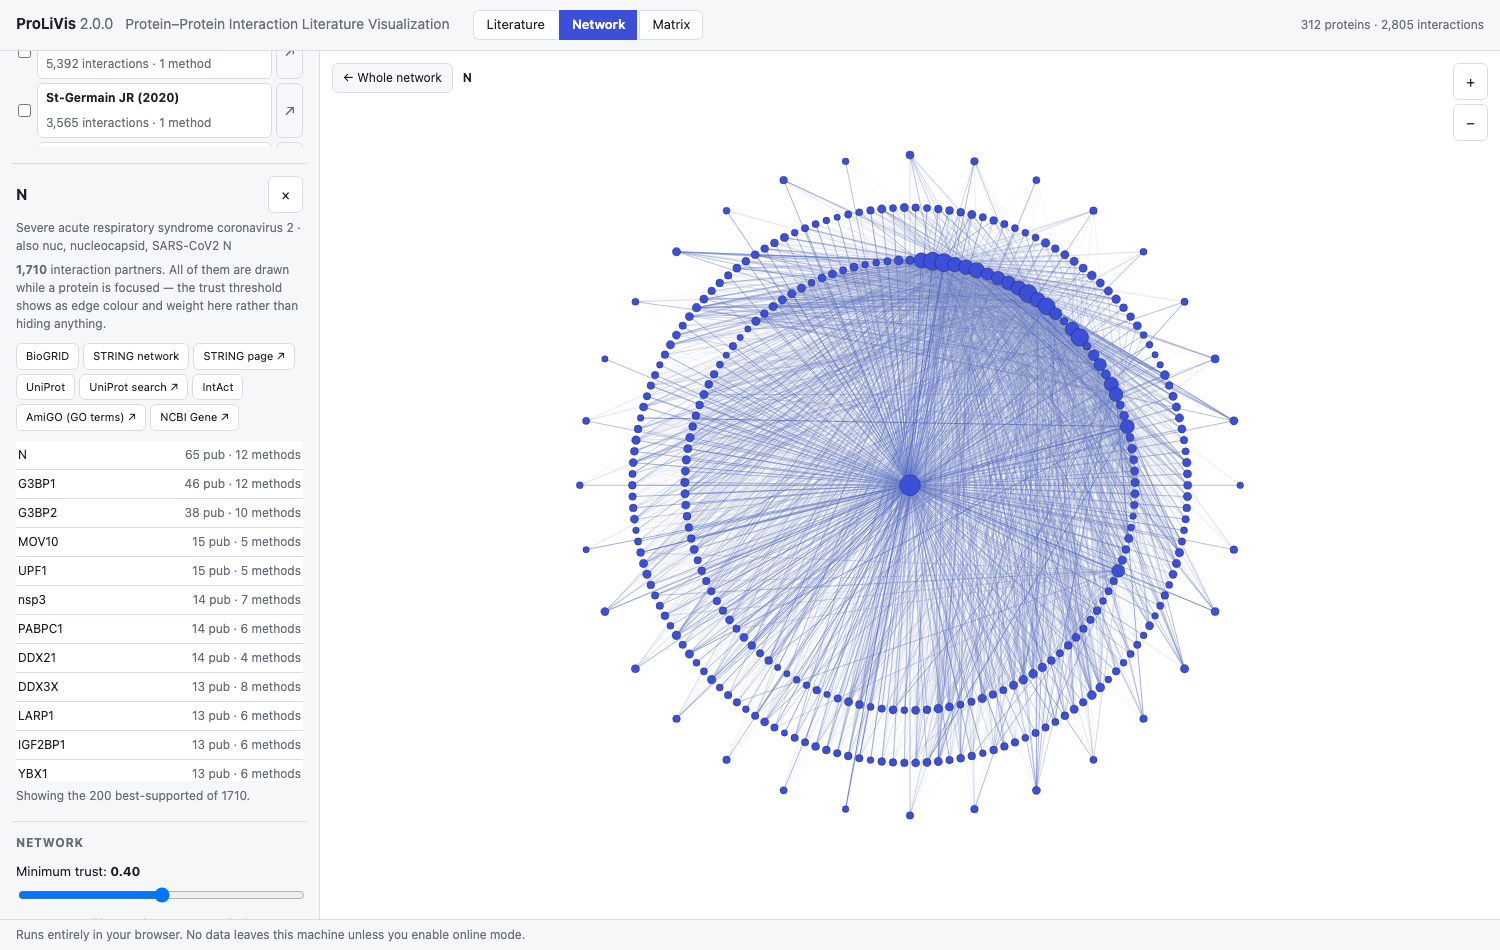
\includegraphics[width=0.86\textwidth]{supplement/protein-panel.png}
  \caption{Clicking a protein centres the view on it and lists every interaction it
  takes part in, with how many publications and how many methods support each. The
  arrangement becomes an ego layout: radius is graph distance, so the picture states
  how each partner is reached. The list says how many of the partners it is showing.}
\end{figure}

\begin{figure}[h]
  \centering
  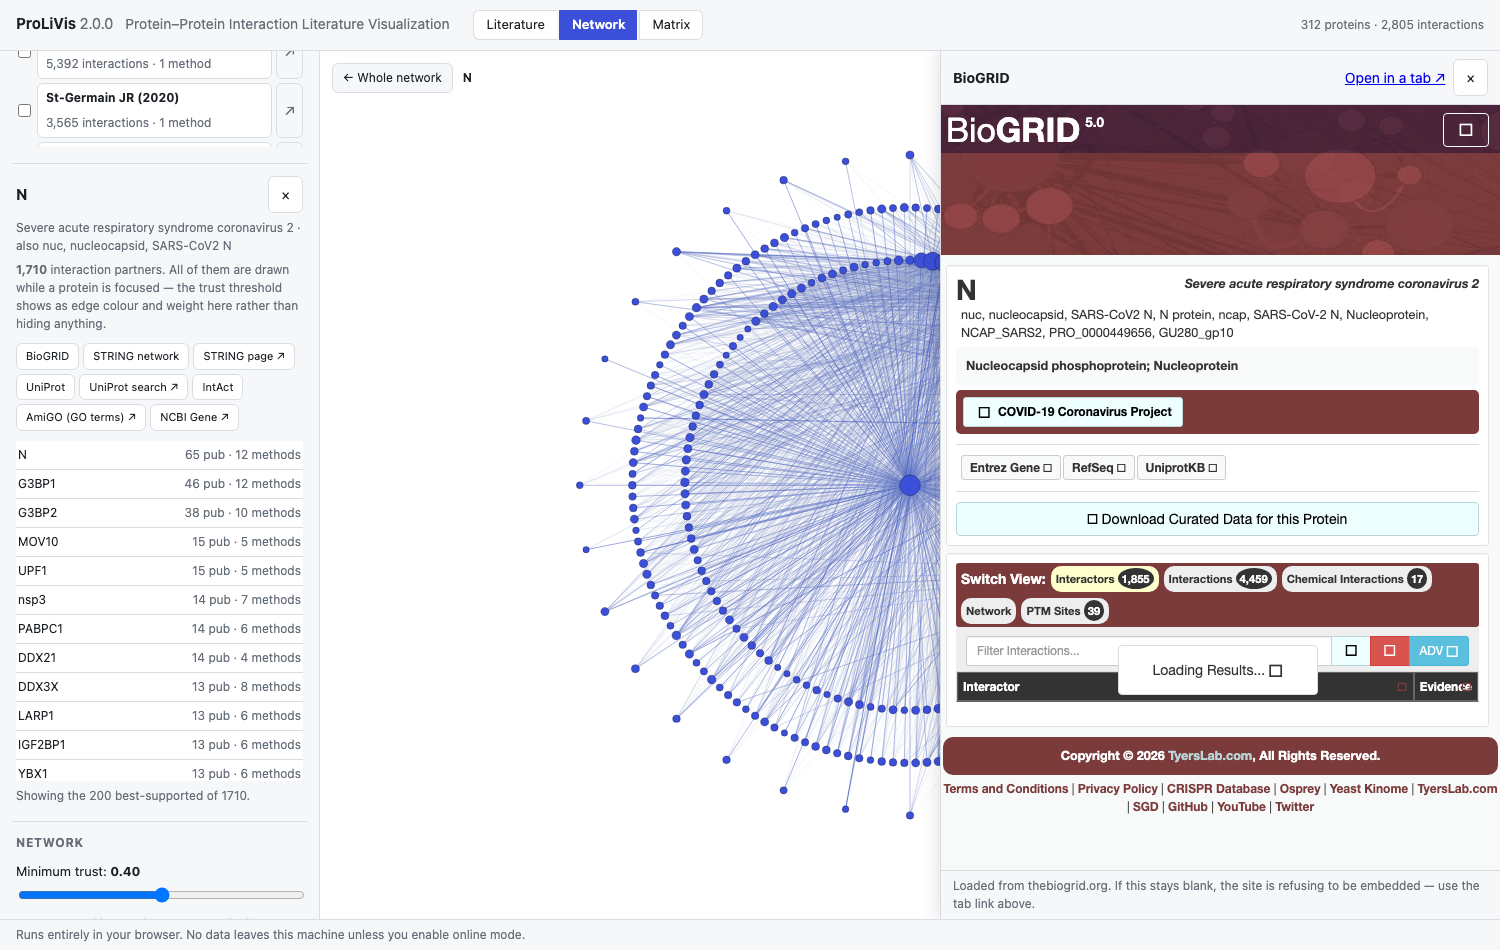
\includegraphics[width=0.86\textwidth]{supplement/external-panel.png}
  \caption{Links out to BioGRID, STRING, UniProt, IntAct, AmiGO and NCBI Gene. Where a
  site permits framing its page opens beside the network; where it does not, the link
  opens a tab, and STRING's network image is shown instead. The list is editable: a
  base URL and a template over \texttt{\{symbol\}}, \texttt{\{biogridId\}},
  \texttt{\{entrez\}}, \texttt{\{swissprot\}} and \texttt{\{organismId\}}. Nothing is
  contacted until a link is clicked.}
\end{figure}

\clearpage
\section{Reading a network one level up}
\label{sec:modules}

\begin{figure}[h]
  \centering
  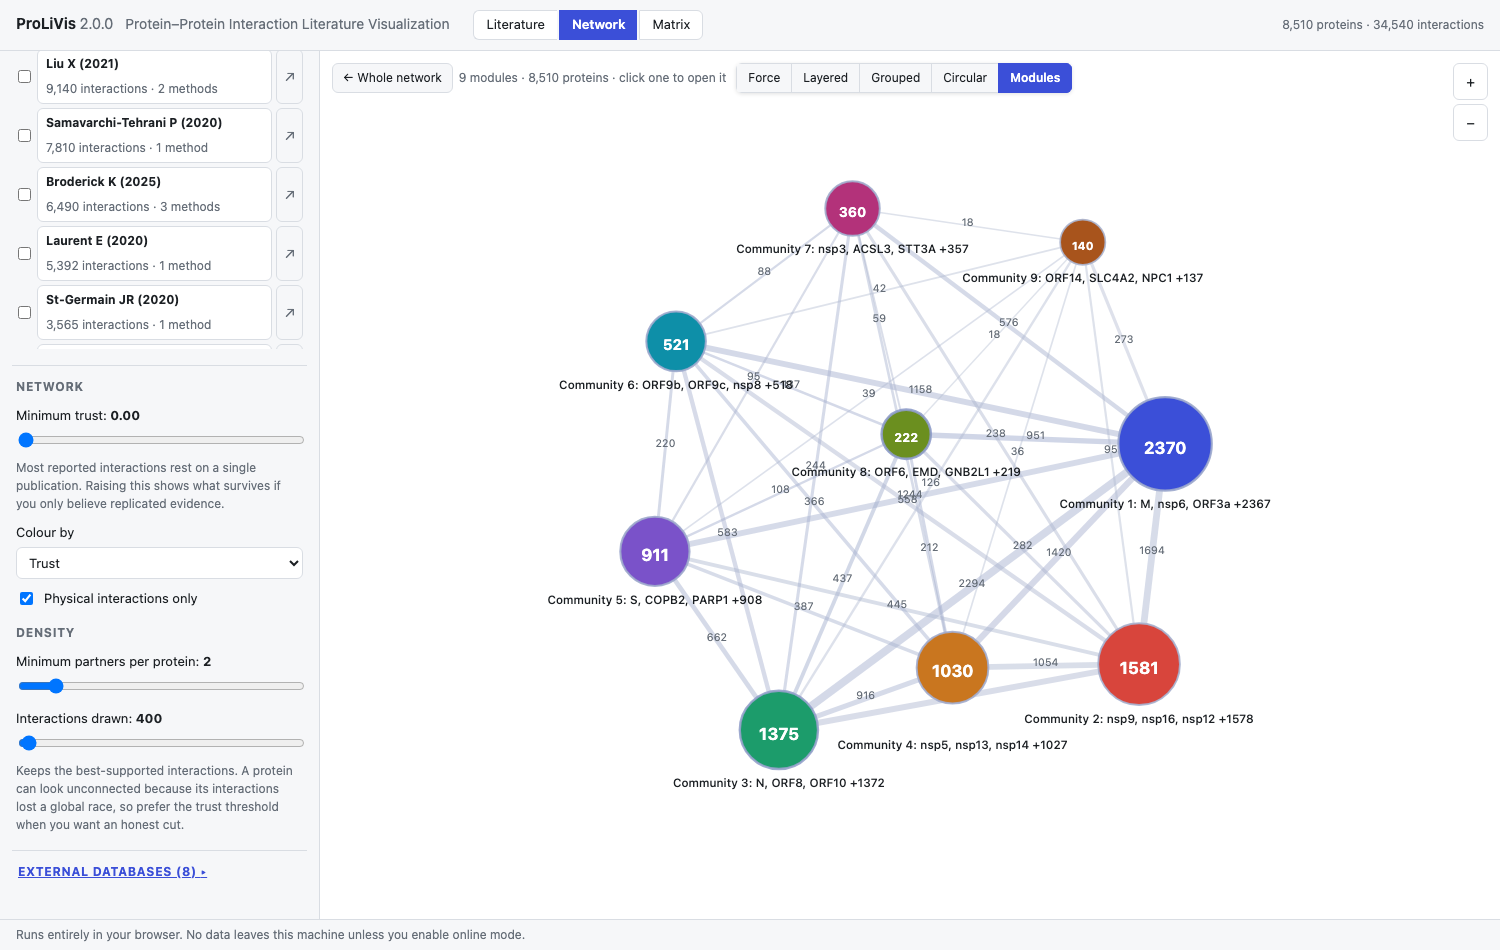
\includegraphics[width=0.86\textwidth]{supplement/modules.png}
  \caption{Modules. A node is a set of proteins --- area by membership, the count
  printed inside, the ring the mean trust of its internal interactions --- and a link
  is the evidence spanning two sets. Biconnected components where they decompose the
  network, trust-weighted communities where they do not.}
\end{figure}

\begin{figure}[h]
  \centering
  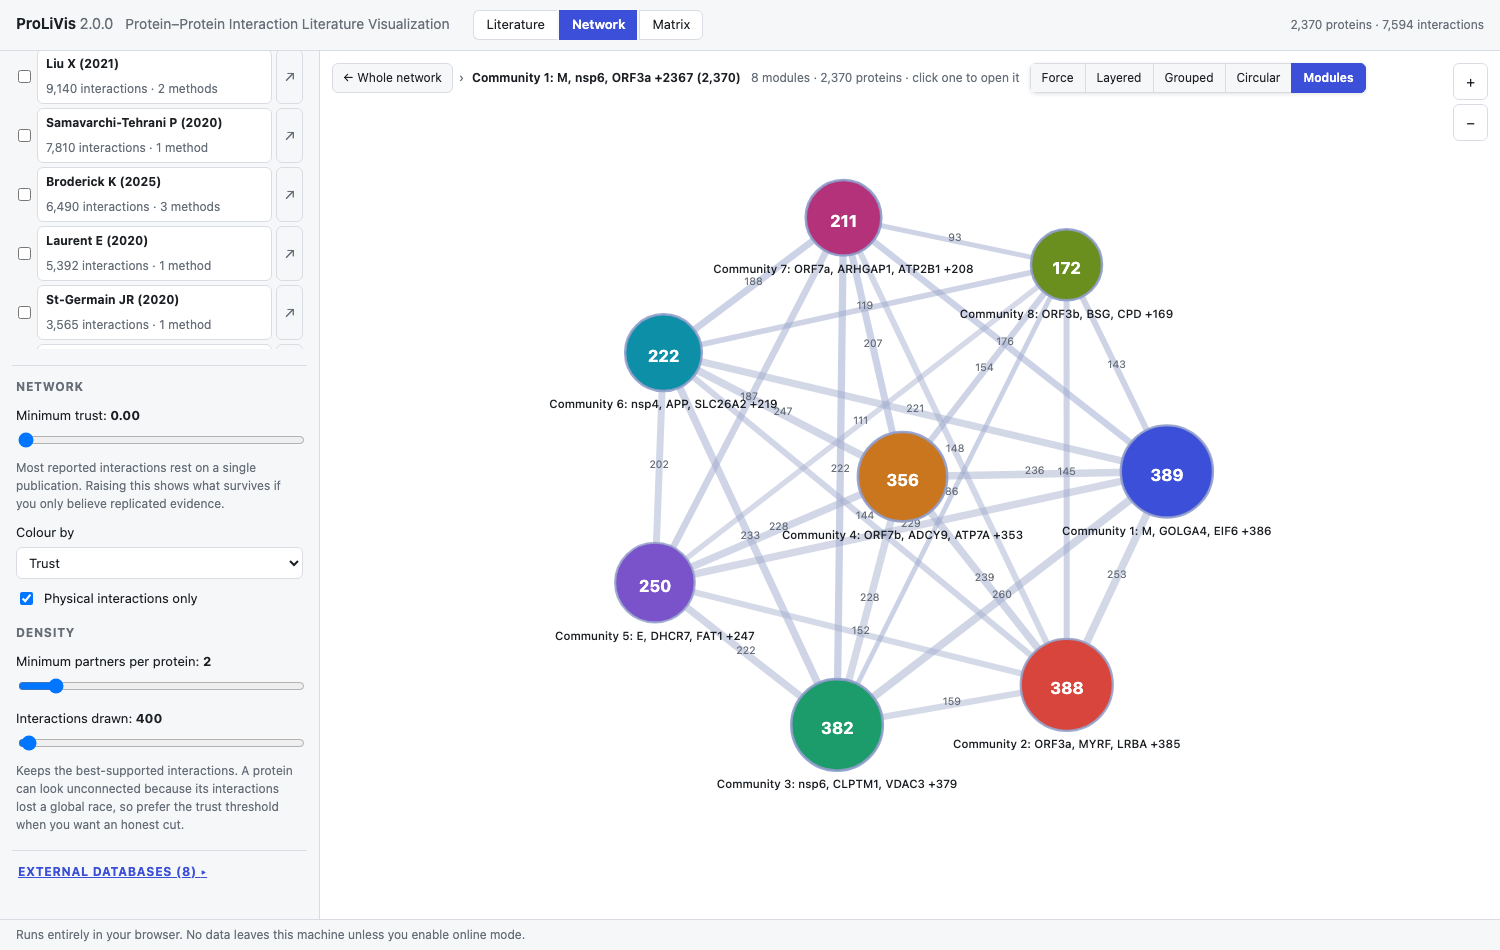
\includegraphics[width=0.86\textwidth]{supplement/modules-drill.png}
  \caption{One module opened. If what is inside is still too large to draw it is
  contracted again, and the breadcrumb grows a level; any level in the trail returns to
  it. On the full human interactome this is four steps from a million interactions to
  53 proteins.}
\end{figure}

\clearpage
\section{The adjacency matrix}

\begin{figure}[h]
  \centering
  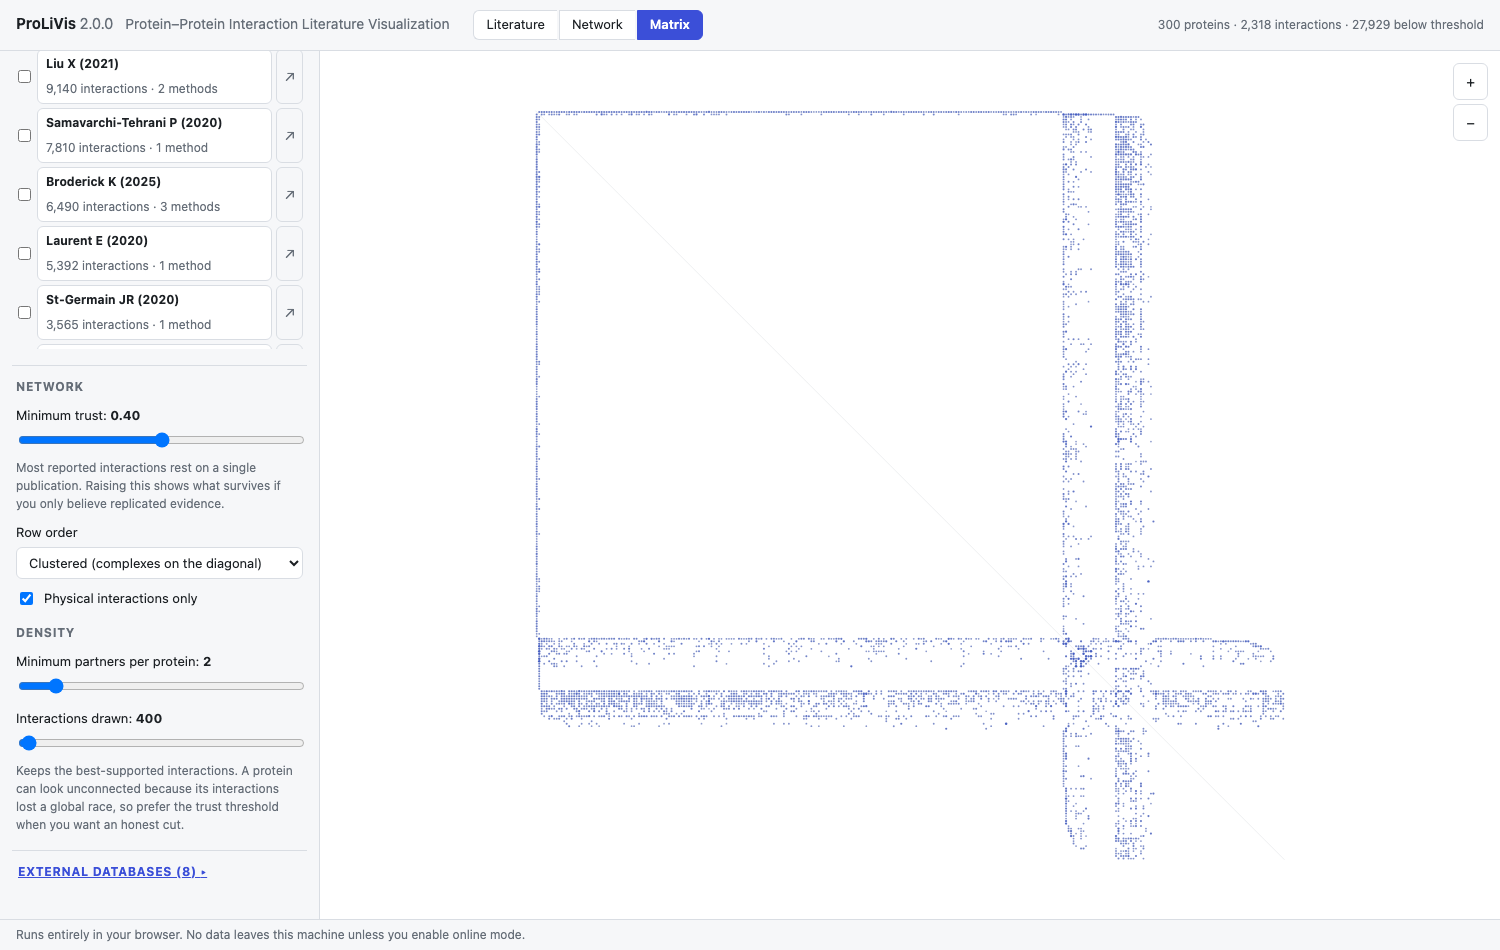
\includegraphics[width=0.86\textwidth]{supplement/matrix.png}
  \caption{The same interactions as a reorderable matrix, coloured by trust. Rows are
  ordered by a breadth-first traversal within components, largest first, visiting the
  highest-degree neighbour first, which puts each module in a contiguous block --- so
  complexes appear as blocks on the diagonal. The matrix is symmetric and both
  triangles are drawn: a triangular plot is more compact and far harder to read one
  protein's row from.}
\end{figure}

\clearpage
\section{Searching the literature, and keeping some of it}

\begin{figure}[h]
  \centering
  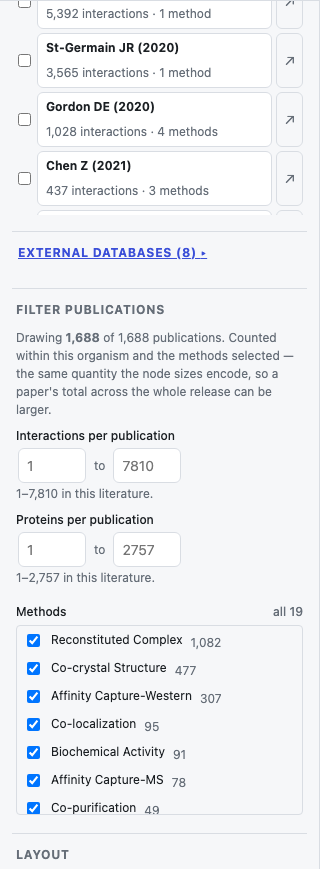
\includegraphics[width=0.42\textwidth]{supplement/literature-search.png}
  \hfill
  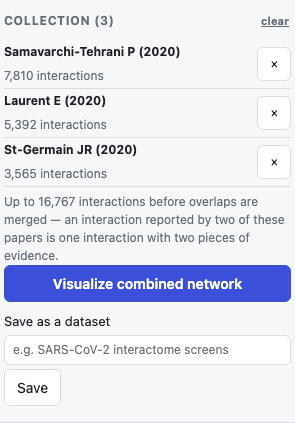
\includegraphics[width=0.42\textwidth]{supplement/collection.png}
  \caption{Search by author, year, PubMed id, DOI or enriched title; with an empty box
  the largest contributors are listed, which answers ``what is this network mostly made
  of''. Each hit says how many interactions and how many methods it contributed before
  you commit to opening it. Ticking hits builds a collection that survives further
  searches.}
\end{figure}

\begin{figure}[h]
  \centering
  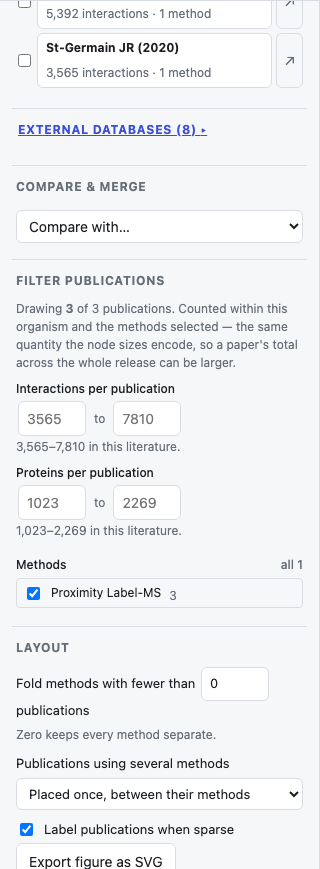
\includegraphics[width=0.42\textwidth]{supplement/derived-dataset.png}
  \hfill
  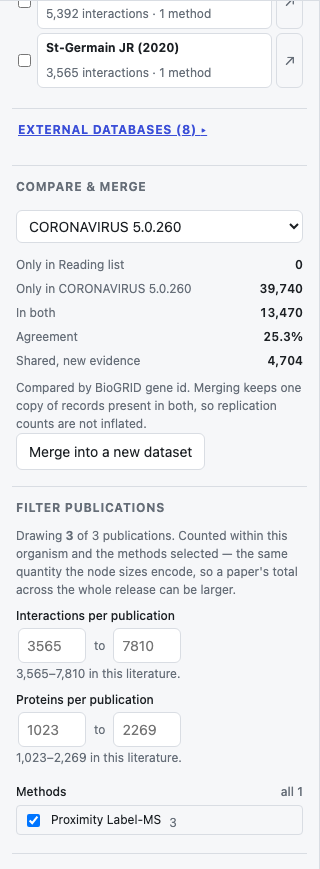
\includegraphics[width=0.42\textwidth]{supplement/compare.png}
  \caption{A collection saved as a dataset of its own --- scorable, comparable,
  exportable, and remembering which publications produced it --- and then compared with
  the release it came from. Records are copied rather than referenced, so removing the
  source cannot change a figure built from the derived set, and overlapping evidence is
  merged rather than counted twice.}
\end{figure}

\clearpage
\section{Views computed but not drawn}
\label{sec:undrawn}

Four view models are implemented, tested and reachable from the API, but the interface
does not yet draw them. They are listed here with their real output rather than
described, and the honest summary is that they are data, not pictures.

\begin{table}[h]
  \centering
  \small
  \caption{\texttt{upset}: which combinations of methods actually support an
  interaction. Most interactions rest on exactly one method; the largest intersection
  is the two mass-spectrometry techniques agreeing.}
  \begin{tabular}{lr}
    \toprule Method combination & Interactions \\ \midrule
    \SuppUpset
    \bottomrule
  \end{tabular}
\end{table}

\begin{table}[h]
  \centering
  \small
  \caption{\texttt{timeline}: when the evidence arrived, by method, over
  \SuppYearFirst--\SuppYearLast. The two dominant methods peak in 2020 and 2021, which
  is what a pandemic looks like in a database.}
  \begin{tabular}{lrr}
    \toprule Method & Interactions & Peak year \\ \midrule
    \SuppTimeline
    \bottomrule
  \end{tabular}
\end{table}

\begin{table}[h]
  \centering
  \small
  \caption{\texttt{methodChord}: which methods support the same interactions.}
  \begin{tabular}{llr}
    \toprule Method & Method & Shared interactions \\ \midrule
    \SuppChord
    \bottomrule
  \end{tabular}
\end{table}

\texttt{bipartite} places publications and the proteins they touched on two axes with a
lane per method: over the twelve largest publications here it produces
\SuppBipartiteNodes{} nodes, \SuppBipartiteLinks{} links and \SuppBipartiteLanes{}
lanes, and reports that it truncated. Each of these takes an assembled input, and the
API produces those inputs from a query (\texttt{pairSystems}, \texttt{timelineRecords},
\texttt{bipartiteInput}).

\clearpage
\section{The trust model, and what can be done with it}

Every interaction is scored from seven terms; the manuscript gives the equations. What
matters in use:

\begin{itemize}
  \item Terms whose inputs are unknown are reported as \emph{unknown}, not as zero, and
        the remaining weights are renormalized. A \texttt{coverage} figure accompanies
        every score, saying how much of the model was informed.
  \item Three presets ship: \texttt{evidence-only} (fully offline),
        \texttt{literature-aware} (the default) and \texttt{structural-strict}.
  \item Re-weighting is instant, because evidence is gathered once and scoring is
        arithmetic over it --- \texttt{gather} then \texttt{rescore}.
  \item \texttt{calibrate} and \texttt{ablate} measure a configuration against a
        reference set of known interactions, reporting AUROC, average precision and a
        leave-one-term-out ablation. The manuscript does not report numbers from these
        because that needs an external reference set; the harness is here.
\end{itemize}

\begin{verbatim}
  const gathered = await prolivis.gather({ datasetId, organismId: 2697049 })
  const strict   = prolivis.rescore(gathered, 'structural-strict')
  const custom   = prolivis.rescore(gathered, { weights: { independence: 0.4 } })
\end{verbatim}

\section{Structure, and what survives the evidence}

All of these are API-level and all take the graph built at a chosen trust threshold, so
every structural question can be asked of ``the network I actually believe''.

\begin{verbatim}
  const graph = await prolivis.graph({ datasetId }, { minScore: 0.4 })

  prolivis.cliques(graph, { minSize: 3 })   // candidate complexes
  prolivis.modules(graph)                   // biconnected components,
                                            // articulation points, bridges
  prolivis.cores(graph)                     // k-core decomposition
  prolivis.communities(graph)               // Louvain, trust-weighted
  prolivis.autoContract(graph)              // what the Modules view draws
  prolivis.removeEdges(graph, 'trust-ascending')
\end{verbatim}

Edge removal comes in two orders. \texttt{betweenness} is classical Girvan--Newman and
asks where the joins are. \texttt{trust-ascending} removes the least-supported edge
first and asks what survives if only the evidence is believed; both record component
count and modularity at every step.

\section{Export, and reproducing a figure}

\begin{verbatim}
  prolivis.exportTable(scored, 'csv')   // a column per trust term
  prolivis.exportSif(scored)            // Cytoscape
  prolivis.exportGraphml(graph)         // typed attributes
  prolivis.toSvg(scene, 'title')        // the picture, as vector

  const manifest = prolivis.manifest({
    dataset, query, trust, layout, publicationFilter,
  })
  const text = prolivis.serializeManifest(manifest)
\end{verbatim}

The manifest records the release, the query, the filters, the trust configuration and
the layout options. With a deterministic layout that is sufficient to regenerate a
figure exactly --- which ProLiVis 1.0 could not do even for its own author, its layout
engine having been an external binary that is now lost. \texttt{checkManifest} reports
whether the loaded datasets can reproduce a given manifest, naming what differs.

\section{Known gaps}

Stated rather than left to be discovered:

\begin{itemize}
  \item Online mode against the BioGRID REST service exists in the API but has no
        panel in the interface; an access key cannot yet be entered by hand.
  \item Data export (CSV, GraphML, GML, SIF) and the session manifest are API-only. The
        interface exports the figure as SVG.
  \item Trust weights are editable through the API but not in the interface, which
        offers the threshold slider and the shipped presets' behaviour only.
  \item UpSet, timeline, chord and bipartite are computed but not drawn
        (\S\ref{sec:undrawn}).
  \item Literature enrichment covers OpenAlex with PubMed as a fallback; publications
        neither resolves leave the two bibliometric terms unknown, which the coverage
        figure reports.
\end{itemize}

\end{document}
